%% Preambel
\documentclass[conference,compsoc,final,a4paper]{IEEEtran}
\usepackage[utf8]{inputenx}

%% Bitte legen Sie hier den Titel und den Autor der Arbeit fest
\newcommand{\autoren}[0]{Cöllen, Markus}
\newcommand{\dokumententitel}[0]{Kann Malware in Android-Apps automatisch gefunden
werden?}

% Hie muss normalerweise nichts angepasst werden
\usepackage[pdftex]{graphicx}
\graphicspath{{img/}}
\DeclareGraphicsExtensions{.pdf,.jpeg,.jpg,.png}
\usepackage[cmex10]{amsmath}
\usepackage{algorithmic}
\usepackage{array}
\usepackage{dblfloatfix}
\usepackage{url}
\usepackage[autostyle=true,german=quotes]{csquotes}
\usepackage[backend=bibtex]{biblatex}
\usepackage{booktabs}
\usepackage{xcolor}
\usepackage{listings}             % Source Code listings
\usepackage[printonlyused]{acronym}

% Farben definieren
\definecolor{linkblue}{RGB}{0, 0, 100}
\definecolor{linkblack}{RGB}{0, 0, 0}
\definecolor{darkgreen}{RGB}{14, 144, 102}
\definecolor{darkblue}{RGB}{0,0,168}
\definecolor{darkred}{RGB}{128,0,0}
\definecolor{comment}{RGB}{63, 127, 95}
\definecolor{javadoccomment}{RGB}{63, 95, 191}
\definecolor{keyword}{RGB}{108, 0, 67}
\definecolor{type}{RGB}{0, 0, 0}
\definecolor{method}{RGB}{0, 0, 0}
\definecolor{variable}{RGB}{0, 0, 0}
\definecolor{literal}{RGB}{31,0, 255}
\definecolor{operator}{RGB}{0, 0, 0}

\usepackage[ngerman]{betababel}
\usepackage[
	    unicode=true,
      hypertexnames=false,
      colorlinks=true,
      colorlinks=false,
      linkcolor=darkblue,
      citecolor=darkblue,
      urlcolor=darkblue,
      pdftex
   ]{hyperref}
%	 \PrerenderUnicode{ü}

% Einstellungen für Quelltexte
\lstset{
      xleftmargin=0.1cm,
      basicstyle=\scriptsize\ttfamily,
      keywordstyle=\color{keyword},
      identifierstyle=\color{variable},
      commentstyle=\color{comment},
      stringstyle=\color{literal},
      tabsize=2,
      lineskip={2pt},
      columns=flexible,
      inputencoding=utf8,
      captionpos=b,
      breakautoindent=true,
	  breakindent=2em,
	  breaklines=true,
	  prebreak=,
	  postbreak=,
      numbers=none,
      numberstyle=\tiny,
      showspaces=false,      % Keine Leerzeichensymbole
      showtabs=false,        % Keine Tabsymbole
      showstringspaces=false,% Leerzeichen in Strings
      morecomment=[s][\color{javadoccomment}]{/**}{*/},
      literate={Ö}{{\"O}}1 {Ä}{{\"A}}1 {Ü}{{\"U}}1 {ß}{{\ss}}2 {ü}{{\"u}}1 {ä}{{\"a}}1 {ö}{{\"o}}1
}

\hypersetup{
  pdftitle={\dokumententitel},
	pdfauthor={\autoren},
	pdfdisplaydoctitle=true
}

% Wo liegt Sourcecode?
\newcommand{\srcloc}{src/}

% Literatur einbinden
\addbibresource{literatur.bib}

\begin{document}

% Titel des Dokuments
\title{\dokumententitel}

% Namen der Autoren
\author{
  \IEEEauthorblockN{\autoren}
  \IEEEauthorblockA{
    Hochschule Mannheim\\
    Fakultät für Informatik\\
    Paul-Wittsack-Str. 10,
    68163 Mannheim
    }
}

% Titel erzeugen
\maketitle
\thispagestyle{plain}
\pagestyle{plain}
 % Weitere Einstellungen aus einer anderen Datei lesen

% Eigentliches Dokument beginnt hier
% ----------------------------------------------------------------------------------------------------------

% Kurze Zusammenfassung des Dokuments
\begin{abstract}
An dieser Stelle steht eine kurze Zusammenfassung des Inhaltes des Dokuments.
\end{abstract}

\tableofcontents

\section{Einleitung}

\section{Grundlagen}

\subsection{Android als Ziel}
Smartphones bieten aufgrund ihrer vielen Schittstellen zur Außenwelt, wie z.B. WLAN, Bluetooth, NFC, USB usw. viele Angriffspunkte. Ein Hauptgrund, warum Smartphones mit dem Android Betriebssystem so beliebt für Angreifer sind, ist der hohe Verbreitungsgrad dieser Geräte. Dieser liegt im Jahr 2018 bei ca. 86 Prozent und ist somit Sechs mal so hoch wie der Konkurrent IOS mit knapp 16 Prozent Marktanteil \cite{AndoidMarktanteil}. Weil Android unter der Apache Open-Source Lizenz freigegeben ist und das Betriebssystem auf dem Linux-Kernel basiert, können Hersteller das Android Betriebssystem beliebig verwenden und für ihre Produkte anpassen. Zudem dient der Linux-Kernel als eine Abstraktion zwischen Software und Hardware und somit kann Android auf verschiedenen Geräten eingesetzt werden. Aufgrund der Tatsache, dass Linux über ein etabliertes Sicherheitskonzept verfügt \cite{LinuxSicherheitskonzept}, greift Android auf viele Schutzmechanismen des Linux Kernels
zurück oder benutzt diese als ihre Basis 
\cite{scheid2012kapitel}.

\subsection{Android Update Problematik}\label{sec:Android Update Problematik}

Wie man in Abbildung \ref{fig_sim} sehen kann verdrängen die neueren Android Versionen die älteren. Allerdings ist Android Oreo, mit gerade mal 4,6 Prozent, eine der am wenigsten vertretenen Version, obwohl sie die neueste und auch schon seit dem 27. August 2017 auf dem Markt ist. 

\begin{figure}[!ht]
\centering
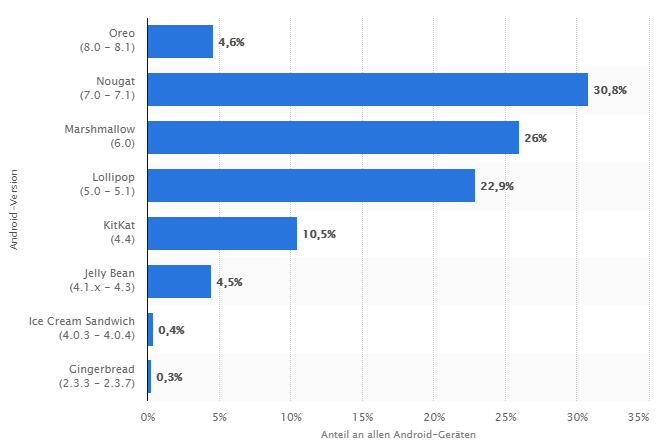
\includegraphics[width=8.5cm]{AndroidVersionen2}
\caption{Android-Versionen~\cite{Android-Versionen}}
\label{fig_sim}
\end{figure}

Dies liegt daran, dass nicht jede Android Version mit jedem Handy kompatibel ist. Die Smartphone Hersteller müssen die Versionen an ihre Geräte und die jeweilige Hardware anpassen. Diese umfassen Anpassungen an WLAN, Kamera, Bluetooth, GPS  usw. Anschließend müssen die erstellten Anpassungen noch umfangreich getestet werden, was auch noch viel Zeit in Anspruch nimmt. Weil die Hersteller oft neue Produkte verkaufen wollen und das Updaten älterer Smartphones zu teuer und zeitaufwendig ist, bleibt den Nutzern oft nichts anderes übrig, als neue Smartphones zu kaufen. Andernfalls behält man ein Smartphone mit einer veralteten Version und bekannten Sicherheitslücken. \cite{scheid2012kapitel}.  

\subsection{Application Sandbox}
\label{sec:Application Sandbox}
Linux arbeitet als ein Mehrbenutzer-Betriebssystem. Dies bedeutet, dass es mehrere Nutzer geben kann und das Betriebssystem verhindert, dass Daten eines Nutzers von einem anderen Nutzer eingesehen, geändert oder gelöscht werden können. Diese Nutzermanagement wird beim Application Sanboxing verwendet. Hierbei erhält jede Applikation eine eigene Nutzer-ID und führt diese in einem separaten Prozess aus. Somit gewährleistet Android, dass eine Applikation anderen Applikationen oder dem Betriebssystem keinen Schaden zufügen kann. Sollte eine Applikation aber durch das Ausnutzen einer Schwachstelle oder einer Sicherheitslücke an Root-Rechte kommen, kann die Applikation dieses Application Sanboxing einfach umgehen. Wie schon in Abschnitt \ref{Android Update Problematik} beschrieben, gibt es wegen den stark verzögerten Android Updates oft Sicherheitslücken, welche über längere Zeit bekannt sind und leicht ausgenutzt werden können um Root-Rechte zu erlangen \cite{scheid2012kapitel}.

\subsection{Permission Model}
\label{sec:Permission Model}
Standardmäßig hat eine Applikation keinen Zugriff auf Daten außerhalb der Sandbox. Sollte eine Applikation Systemressourcen außerhalb dieser verwenden wollen, muss erst eine Zugriffsanfrage gestellt werden. Geschützte Ressourcen sind z.B. Kamera, SMS, Bluetooth usw. \cite{PermissonModel}. Diese Rechte können allerdings nur angenommen oder abgelehnt werden. 

\subsection{Google Play Store}
Anders als bei IOS, bei welchem die Nutzer an den Apple Store gebunden sind, können die Android Benutzer selbst entscheiden welchen Store sie verwenden. Der Google Play Store ist mit 82 Milliarden Downloads  \cite{GooglePlayDownloads} mit Abstand die größte Plattform. Er wurde am 28. August 2008 unter dem Namen Android Market veröffentlicht. Dieser bietet den Nutzern einfaches herunterladen und installieren von mobilen Anwendungen, sogenannten Applikationen. Im Google Play Store sind inzwischen über 3,7 Millionen Anwendungen  bereit zum Herunterladen \cite{Apps} und jeden Monat kommen ca. 30.000 neue Applikationen hinzu \cite{bartsch2014zertifizierte}. Durch den rasanten Wachstum steigt auch die Anzahl von schädlicher Software, sogenannter Malware. Der Anteil von bösartigen Applikationen ist von 2011 bis 2013 um 388\% gewachsen \cite{RiskIQ}. Da nicht alle Anwendungen von Mitarbeitern geprüft werden können, hat Google das Programm Bouncer ins Leben gerufen (siehe Kapitel \ref{sec:Bouncer}).
Android bietet zudem die Möglichkeit per Remote-Verbindung Applikationen zu installieren und zu löschen. Hierfür braucht man lediglich Zugriff auf den Google Play Account. Falls ein Angreifer an diese Daten kommen sollte, könnte er ohne Erlaubnis des Nutzers, Applikationen aus dem Google Play Store auf dem Smartphone installieren.
\subsection{Malware}
Der Begriff Malware steht für malicous software und bezeichnet Programme, welche unerwünschte oder auch schädliche Funktionen ausführen. Sie stellen eine immer größer werdende Bedrohung dar und durch den rasanten Wachstum ist eine manuelle Auswertung mittlerweile unmöglich geworden. Obwohl es sich bei vielen neuen Arten um verschiedene Varianten bereits bekannter Malware handelt, müssen Analysten erst jedes Sample erneut analysieren um dies feststellen zu können \cite{trinius2010visualisierung}. Bei der Analyse kann grundsätzlich in zwei Arten unterschieden werden: Statische und Dynamische Analyse (siehe Kapitel \ref{sec:Statische Analyse} und \ref{sec:Dynamische Analyse}).


\section{Analysemethoden}

\subsection{Statische Analyse} \label{sec:Statische Analyse}

\subsubsection{Data Flow}

\subsubsection{Control Flow}

\subsection{Dynamische Analyse} \label{sec:Dynamische Analyse}

\section{Bouncer} \label{sec:Bouncer}

\section{Fazit}

 Eine Abkürzung = \ac{A2A} 


%% --------------------------------------------------------------------

\section*{Abkürzungen}
\addcontentsline{toc}{section}{Abkürzungen}

\begin{acronym}
\acro{A2A}{Application-to-Application}
\end{acronym}

% Literaturverzeichnis
\addcontentsline{toc}{section}{Literatur}
\printbibliography

\end{document}
